\chapter{Implementierung}
\label{cha:Implementierung}
Zum Beweis wurde für die Firma BMD ein Prototyp implementiert. 
Dieser soll zeigen, dass mit der genannten strukturellen Vorgehensweise möglich ist, ohne großen Wartungsaufwand Schemadateien zu generieren.


\section{Allgemein}
Die Implementierung des Schemagenerators wurde mit Delphi realisiert. 
Als Basis für die Umsetzung wurde betriebsinterne Funktionen zum Schreiben von XML-Dokumenten verwendet. 
Diese werden im Unternehmen bereits seit mehreren Jahren verwendet und ausreichend getestet.
Ziel war es hier eine Mischung von einer generischen Umsetzung und kundenspezifischer Lösung zu finden. 
Deswegen wurde explizite Funktionen eingebaut, wo einige wenige Sonderfälle behandelt werden können.


\begin{figure}
    \centering
    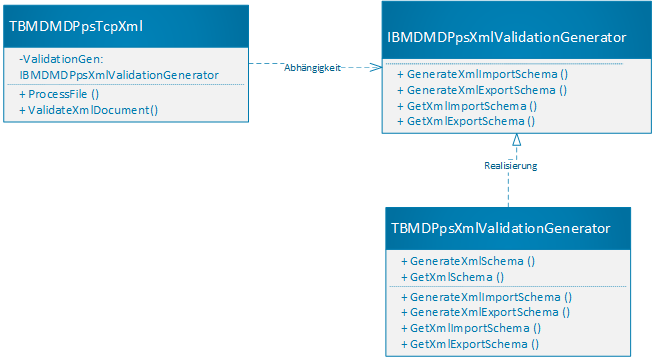
\includegraphics[width=.95\textwidth]{images/KlassenUML.png}
    \caption{Klassen-Aufbau}
    \label{fig:Klassenaufbau}
\end{figure}

\section{XML Schema}
Die Generierung des Schemas kann über zwei Arten erfolgen. 
Entweder wird das Schema nur im Programmspeicher der Anwendung angelegt und zur Validierung im System verwendet, oder das Schema wird auf einem definierten Speicherort abgelegt. Siehe Abbildung \ref{fig:Schemas}.

Das Schema besteht dann im Detail aus zumindest einem Wurzel-Element in dem dann alle zulässigen Typen definiert werden können. Die definierten Typen werden über \emph{complexType}-Elemente abgebildet. Da diese wiederum weitere Typen enthalten können, kann sich diese Methode rekursiv aufrufen. Siehe Abbildung \ref{fig:SchemaF}.

Danach können noch etwaige Spezialfälle hinzugefügt werden. Diese sind leider bereits von bestehenden Schnittstellen vorgegeben und müssen auch in Zukunft gewartet und erweitert werden können. Siehe Abbildung \ref{fig:SchemaE}.
 
% \ref{fig:Schemas}

% \begin{quote}
% \begin{verbatim}
% \begin{GenericCode}
% \end{GenericCode}
% \end{verbatim}
% \end{quote}
% einstellen von Programiersprache, Format, ...
\begin{figure}
\lstset{language=Pascal, 
        basicstyle=\tiny\ttfamily, 
        numbers=left,
        numberstyle=\tiny, 
        stepnumber=5, 
        firstnumber=0,
        showstringspaces=false}
\lstinputlisting {images/Schema.pas}
\caption{Erstellung des Schemas.}
% \caption{Erstellung des Schemas.}
 \label{fig:Schemas}
 \end{figure}
 
\begin{figure}
\lstset{language=Pascal, 
        basicstyle=\tiny\ttfamily, 
        numbers=left,
        numberstyle=\tiny, 
        stepnumber=5, 
        firstnumber=0,
        showstringspaces=false}
\lstinputlisting {images/Schema2.pas}
\caption{Erstellung des Schemas - Fortsetzung.}
% \caption{Erstellung des Schemas - Fortsetzung.}
 \label{fig:SchemaF}
 \end{figure}
 
\begin{figure}
\lstset{language=Pascal, 
        basicstyle=\tiny\ttfamily, 
        numbers=left,
        numberstyle=\tiny, 
        stepnumber=5, 
        firstnumber=0,
        showstringspaces=false}
\lstinputlisting {images/Schema3.pas}
\caption{Erstellung des Schemas - Ende.}
% \caption{Erstellung des Schemas - Ende.}
 \label{fig:SchemaE}
 \end{figure}

\section{XML Schematron}
Das Schematron besteht aus fix definierten Regeln, die immer kontextspezifisch sind. 
Deswegen muss für jede Schnittstelle die Regeln eigens implementiert werden.
Bei der Erstellung des XML Schemas wird aufgrund von fix definierten Kennzahlen ermittelt, ob für diese Schnittstelle ein Schematron umgesetzt wurde und angefügt werden soll. 
Siehe dazu Abbildung \ref{fig:Schematron}.

\begin{figure}
\lstset{language=Pascal, 
        basicstyle=\tiny\ttfamily, 
        numbers=left,
        numberstyle=\tiny, 
        stepnumber=5, 
        firstnumber=0,
        showstringspaces=false
        %,commentstyle=\color{OliveGreen}
        }
\lstinputlisting {images/Schematron.pas}
\caption{Erstellung des Schematron.}
\label{fig:Schematron}
\end{figure}


Wenn für diese Schnittstelle eine oder mehrere Regel definiert wurden, so wird mittels der \emph{AddPattern}-Funktion, siehe Abbildung \ref{fig:Schematron2} und der \emph{AddRule}-Funktion, siehe Abbildung \ref{fig:Schematron3}, die notwendigen Annotationen eingefügt. 

\begin{figure}
\lstset{language=Pascal, 
        basicstyle=\tiny\ttfamily, 
        numbers=left,
        numberstyle=\tiny, 
        stepnumber=5, 
        firstnumber=0,
        showstringspaces=false}
\lstinputlisting {images/Schematron2.pas}
\caption{Erstellung eines Pattern.}
\label{fig:Schematron2}
\end{figure}

\begin{figure}
\lstset{language=Pascal, 
        basicstyle=\tiny\ttfamily, 
        numbers=left,
        numberstyle=\tiny, 
        stepnumber=5, 
        firstnumber=0,
        showstringspaces=false}
\lstinputlisting {images/Schematron3.pas}
\caption{Erstellung einer Regel.}
\label{fig:Schematron3}
\end{figure}


\section{Validierung im System}
In Abbildung \ref{fig:ValidationExp} erfolgt die Validierung der Dokumente im System. 
Dies muss am Beginn des Ablaufes stattfinden, da bei einer negativen Validierung ein weiteres Behandeln des Dokuments nicht mehr notwendig und sinnvoll ist. 
Für die Überprüfung des Schemas mit dem XML-Dokument wird das \emph{IXMLDOMDocument2} verwendet.
Dies ist eine Komponente von Microsoft die nach Delphi portiert wurde.


\begin{figure}
% einstellen von Programiersprache, Format, ...
\lstset{language=Pascal, 
        basicstyle=\tiny\ttfamily, 
        numbers=left,
        numberstyle=\tiny, 
        stepnumber=5, 
        firstnumber=0,
        showstringspaces=false}
  % Datei "listing.pas" einbinden
\lstinputlisting
    %[caption=Mein Delphi-Code}, label=lst:delphi-code]
    {images/validation.pas}
\caption{Validierung im System mit Schematron%\cite{ValidationExp}.
}
\label{fig:ValidationExp}

Das Ergebnis der Validierung und etwaige aufgetretene Probleme müssen den Benutzer mitgeteilt werden können.
Deswegen wurden Schnittstellen für die Kommunikation implementiert, mit deren es möglich ist, Meldungen an den Aufrufer zu liefern. Siehe dazu Abbildung \ref{fig:Communication}.
\end{figure}

\begin{figure}
% einstellen von Programiersprache, Format, ...
\lstset{language=pascal, 
        basicstyle=\tiny\ttfamily, 
        numbers=left,
        numberstyle=\tiny, 
        stepnumber=5, 
        firstnumber=0,
        showstringspaces=false}
  % Datei "listing.pas" einbinden
\lstinputlisting
    %[caption=Mein Delphi-Code}, label=lst:delphi-code]
    {images/Communication.pas}
\caption{Kommunikation von Meldungen und Ergebnissen%\cite{Communication}.
}
\label{fig:Communication}
\end{figure}